\section{PHÂN TÍCH ĐA THỨC THÀNH NHÂN TỬ}
\subsection{Phân tích đa thức thành nhân tử bằng cách đặt nhân tử chung}
\subsubsection{Kiến thức trọng tâm}
\begin{tomtat}
	\begin{itemize}
	\item Nếu tất cả các hạng tử của đa thức có một nhân tử chung thì đa thức đó biểu diễn được thành một tích của nhân tử chung đó với một đa thưc khác: $A B+A C+\ldots=A(B+C+\ldots)$. 
	\item Nhân tử chung được xác định như sau
	\begin{itemize}
		\item Phần hệ số thường là ƯCLN của các hệ số (trong trường hợp hệ số là số nguyên).	
		\item Phần biến là các biến chung có mặt trong tất cả các hạng tử với số mũ nhỏ nhất.
	\end{itemize}
\end{itemize}
\end{tomtat}

\begin{vd}%[Dự án EX-9-Đề Cương Toán 8-L1]%[Phạm Hoàng Điệp]%[8D1N4-2]
	Phân tích các đa thức sau thành nhân tử:
	\begin{multicols}{2}
	\begin{enumerate}
		\item $x^3+x$;
		\item $6y^3+2y$;
		\item $2(x+y)-2y(x+y)$;
		\item $4(x-y)-3x(x-y)$.
	\end{enumerate}
	\end{multicols}
	\loigiai{
		\begin{enumerate}
			\item $x^3+x = x \cdot x^2+x=x\left(x^2+1\right)$.
			\item $6y^3+2y=2y\left(3y^2+1\right)$.
			\item $2(x+y)-2y(x+y)=(2-2y) \cdot \left(x+y\right)=2(1-y) \cdot (x+y)$.
			\item $4(x-y)-3x(x-y)=(x-y) \cdot (4-3x)$.
		\end{enumerate}
	}
\end{vd}

\begin{vd}%[Dự án EX-9-Đề Cương Toán 8-L1]%[Phạm Hoàng Điệp]%[8D1H4-2]
	Phân tích các đa thức sau thành nhân tử
	\begin{multicols}{2}
	\begin{enumerate}
		\item $2y(10y-3)-15(3-10y)$;
		\item $3x(x-7y)+24(7y-x)$;
		\item $21x(4x+5)+36x+45$;
		\item $12x-60+5y(5-x)$;
		\item $5x(2y-z)+2x^2y-x^2z$;
		\item $2xy^2-6xyz-10x(3z-y)$.
	\end{enumerate}
	\end{multicols}
	\loigiai{
	\begin{enumerate}
		\item $2y(10y-3)-15(3-10y)=2y(10y-3)+15(10y-3)=(10y-3)(2y+15)$.
		\item  $3x(x-7y)+24(7y-x)=3x(x-7y)-24(x-7y)=3(x-7y)(x-8)$.
		\item $21x(4x+5)+36x+45=21x(4x+5)+9(4x+5)=3(4x+5)(7x+3)$.
		\item  $12x-60+5y(5-x)=-12(5-x)+5y(5-x)=(5-x)(5y-12)$.
		\item $5x(2y-z)+2x^2y-x^2z=5x(2y-z)+x^2(2y-z)=x(2y-z)(x+5)$.
		\item $2xy^2-6xyz-10x(3z-y)=2xy(y-3z)+10x(y-3z)=2x(y-3z)(y+5)$.
	\end{enumerate}
	}
\end{vd}	
\subsubsection{Bài tập}

\begin{bt}%[Dự án EX-9-Đề Cương Toán 8-L1]%[Phạm Hoàng Điệp]%[8D1H4-2]
	Phân tích các đa thức sau thành nhân tử
	\begin{multicols}{2}
	\begin{enumerate}
		\item $4x-12$;
		\item $2y-6$;
		\item $x^2-6x$;
		\item $2y^2-5y^3$;
		\item $3x^2y-6xy^2$;
		\item $5x^2-10x^3$;
		\item $3x^4-27x^3$;
		\item $-8x^3y-16xy^3$;
		\item $2x(x-2)+3(x-2)$;
		\item $-3(2x+1)+5x(2x+1)$;
		\item $4x(7x-3)-5(3-7x)$;
		\item $x(2x-y)+4(y-2x)$;
		\item $2x(y-3)+5(y-3)$;
		\item $y(3+4x)+2x(4x+3)$;
		\item $2y(3y-5)-9(5-3y)$;
		\item $2y(2x-y)-6z(y-2x)$;
		\item $3x(x+4)+4y(x+4)+5(x+4)$.
	\end{enumerate}
	\end{multicols}
	\loigiai{
	\begin{enumerate}
		\item $4x-12=4(x-3)$.
		\item $2y-6=2(y-3)$.
		\item $x^2-6x=x(x-6)$.
		\item $2y^2-5y^3=y^2(2-5y)$.
		\item $3x^2y-6xy^2=3xy(x-2y)$.
		\item $5x^2-10x^3=5x^2(1-2x)$.
		\item $3x^4-27x^3=3x^3(x-9)$.
		\item $-8x^3y-16xy^3=-8xy\left(x^2+2y^2\right)$.
		\item $2x(x-2)+3(x-2)=(x-2)(2x+3)$.
		\item $-3(2x+1)+5x(2x+1)=(2x+1)(5x-3)$.
		\item $4x(7x-3)-5(3-7x)=4x(7x-3)+5(7x-3)=(7x-3)(4x+5)$.
		\item $x(2x-y)+4(y-2x)=x(2x-y)-4(2x-y)=(2x-y)(x-4)$.
		\item  $2x(y-3)+5(y-3)=(y-3)(2x+5)$.
		\item  $y(3+4x)+2x(4x+3)=(4x+3)(y+2x)$.
		\item  $2y(3y-5)-9(5-3y)=2y(3y-5)+9(3y-5)=(3y-5)(2y+9)$.
		\item  $2y(2x-y)+6z(2x-y)=2(2x-y)(y+3z)$.
		\item $3x(x+4)+4y(x+4)+5(x+4)=(x+4)(3x+4y+5)$.
	\end{enumerate}
	}
\end{bt}

\begin{bt}%[Dự án EX-9-Đề Cương Toán 8-L1]%[Phạm Hoàng Điệp]%[8D1H4-2]
	Phân tích các đa thức sau thành nhân tử
	\begin{multicols}{2}
		\begin{enumerate}
			\item $5x(2x+3)+6x+9$;
			\item $4x-16+3y(4-x)$;
			\item $12(y-3)+6y(y-3)-9(3-y)$;
			\item $20x(3x+7)+63+27x$;
			\item $6y-54+y(18-2y)$.
		\end{enumerate}
	\end{multicols}
	\loigiai{
		\begin{enumerate}
			\item $5x(2x+3)+6x+9=5x(2x+3)+3(2x+3)=(2x+3)(5x+3)$.
			\item $4x-16+3y(4-x)=4(x-4)-3y(x-4)=(x-4)(4-3y)$.	
			\item 
			\begin{eqnarray*}
				12(y-3)+6y(y-3)-9(3-y)&=& 12(y-3)+6y(y-3)+9(y-3) \\
				&=&6y(y-3)+21(y-3)=3(y-3)(2y+7).
			\end{eqnarray*}	
			\item $20x(3x+7)+63+27x=20x(3x+7)+9(3x+7)=(3x+7)(20x+9)$.
			\item $6y-54+y(18-2y)=6(y-9)-2y(y-9)=2(y-9)(3-y)$.
		\end{enumerate}
	}
\end{bt}

\subsection{Phân tích đa thức thành nhân tử bằng cách sử dụng hằng đẳng thức}
\subsubsection{Kiến thức trọng tâm}
\begin{tomtat}
	Biến đổi các biểu thức về dạng hằng đẳng thức đã biết.
		\begin{itemize}
			\item $a^2+2ab+b^2=(a+b)^2$.
			\item $a^2-2ab+b^2=(a-b)^2$.
			\item $a^2-b^2=(a+b)(a-b)$.
			\item $(a+b)^3=a^3+3a^2b+3ab^2+b^3$.
			\item $(a-b)^3=a^3-3a^2b+3ab^2-b^3$.
			\item $a^3+b^3=(a+b)\left(a^2-ab+b^2\right)$.
			\item $a^3-b^3=(a-b)\left(a^2+ab+b^2\right)$.
		\end{itemize}
\end{tomtat} 

\begin{vd}%[Dự án EX-9-Đề Cương Toán 8-L1]%[Phạm Hoàng Điệp]%[8D1H4-1]
	Phân tích các đa thức sau thành nhân tử:
	\begin{multicols}{4}
	\begin{enumerate}
		\item $x^2-8x+16$;
		\item $x^2-9$;
		\item $9x^2+12x+4$;
		\item $8x^3-27$.
	\end{enumerate}
	\end{multicols}
	\loigiai{
		\begin{enumerate}
			\item $x^2-8x+16=x^2-2 \cdot x \cdot 4+4^2=(x-4)^2$.
			\item $x^2-9=x^2-3^2=(x-3) \cdot (x+3)$.
			\item $9x^2+12x+4=(3x)^2+2 \cdot 3x \cdot 2+2^2=(3x+2)^2$.
			\item $8x^3-27=(2x)^3-3^3=(2x-3)\cdot (4x^2+6x+9)$.
		\end{enumerate}
	}
\end{vd}

\begin{vd}%[Dự án EX-9-Đề Cương Toán 8-L1]%[Phạm Hoàng Điệp]%[8D1H4-1]
	Phân tích các đa thức sau thành nhân tử:
	\begin{multicols}{3}
	\begin{enumerate}
		\item $(x+1)^2-y^2$;
		\item $x^3+3x^2+3x+1$;
		\item $8x^3-12x^2+6x-1$.
	\end{enumerate}
	\end{multicols}
	\loigiai{
		\begin{enumerate}
			\item $(x+1)^2-y^2=(x+1-y) \cdot (x+1+y)$.
			\item $x^3+3x^2+3x+1=(x+1)^3$
			\item $8x^3-12x^2+6x-1=(2x)^3-3 \cdot (2x)^2 \cdot 1+3 \cdot 2x \cdot 1^2 -1^3=(2x-1)^3$.
		\end{enumerate}
	}
\end{vd}

\subsubsection{Bài tập}

\begin{bt}%[Dự án EX-9-Đề Cương Toán 8-L1]%[Phạm Hoàng Điệp]%[8D1H4-1]
	Phân tích các đa thức thành nhân tử
	\begin{multicols}{4}
		\begin{enumerate}
			\item $x^2-16$;
			\item $x^2+4x+4$;
			\item $9y^2-6y+1$;
			\item $x^3-6x^2+12x-8$.
		\end{enumerate}
	\end{multicols}
	\loigiai{
		\begin{enumerate}
			\item   $x^2-16=x^2-4^2=(x-4)(x+4)$.
			\item  $x^2+4x+4=x^2+2 \cdot x \cdot 2+2^2=(x+2)^2$.
			\item  $9y^2-6y+1=(3y)^2-2 \cdot 3y \cdot 1+1^2=(3y-1)^2$.
			\item  $x^3-6x^2+12x-8=x^3-3 \cdot x^2 \cdot 2+3 \cdot x \cdot 2^2-2^3=(x-2)^3$.
		\end{enumerate}
	}
\end{bt}

\begin{bt}%[Dự án EX-9-Đề Cương Toán 8-L1]%[Phạm Hoàng Điệp]%[8D1H4-1]
	Phân tích các đa thức sau thành nhân tử
	\begin{multicols}{2}
		\begin{enumerate}
			\item $25x^2-4$;
			\item $x^2-12x+36$;
			\item $y^3-8$;
			\item $8x^3+36x^2+54x+27$.
		\end{enumerate}
	\end{multicols}
	\loigiai{
		\begin{enumerate}
			\item $25x^2-4=(5x-2)(5x+2)$.
			\item $x^2-12x+36=(x-6)^2$.
			\item $y^3-8=(y-2)\left(y^2+2y+4\right)$.
			\item $8x^3+36x^2+54x+27=(2x+3)^3$.
		\end{enumerate}
	}
\end{bt}

\begin{bt}%[Dự án EX-9-Đề Cương Toán 8-L1]%[Phạm Hoàng Điệp]%[8D1H4-1]
	Phân tích các đa thức sau thành nhân tử
	\begin{multicols}{2}
		\begin{enumerate}
			\item $(x-3)^2-81$;
			\item $4y^2-(2x-3)^2$;
			\item $(2x-5)^2-(3x-4)^2$;
			\item $(2x-y)^3+(2x+y)^3$.
		\end{enumerate}
	\end{multicols}
	\loigiai{
		\begin{enumerate}
			\item   $(x-3)^2-81=(x-3)^2-9^2=(x-3-9)(x-3+9)=(x-12)(x+6)$.
			\item $4y^2-(2x-3)^2=(2y)^2-(2x-3)^2=(2y-2x+3)(2y+2x-3)$.
			\item 
			\begin{eqnarray*}
				(2x-5)^2-(3x-4)^2&=&[(2x-5)-(3x-4)][(2x-5)+(3x-4)]	\\	
				&=&(2x-5-3x+4)(x-5+3x-4)\\
				&=&(-x-1)(5x-9).
			\end{eqnarray*}
			\item  	
			\begin{eqnarray*}
				(2x-y)^3+(2x+y)^3 &=&[(2x-y)+(2x+y)]\left[(2x-y)^2-(2x-y)(2x+y)+(2x+y)^2\right] \\
				&=& (2x-y+2x+y)\left[4x^2-4xy+y^2-\left(4x^2-y^2\right)+\left(4x^2+4xy+y^2\right)\right] \\
				&=& 4x\left(4x^2-4xy+y^2-4x^2+y^2+4x^2+4xy+y^2\right) \\
				&=&4x\left(4x^2+3y^2\right).
			\end{eqnarray*}	
		\end{enumerate}
	}
\end{bt}

\begin{bt}%[Dự án EX-9-Đề Cương Toán 8-L1]%[Phạm Hoàng Điệp]%[8D1H4-1]
	Phân tích các đa thức sau thành nhân tử
	\begin{multicols}{2}
		\begin{enumerate}
			\item  $225-(4-x)^2$;
			\item $(2y+5)^2-9x^2$;
			\item $(3y-4)^2-(2y+5)^2$;
			\item $(z-3y)^3-(z+3y)^3$.
		\end{enumerate}
	\end{multicols}
	\loigiai{
		\begin{enumerate}
			\item  $225-(4-x)^2=(11+x)(19-x)$.
			\item  $(2y+5)^2-9x^2=(2y+5-3x)(2y+5+3x)$.
			\item $(3y-4)^2-(2y+5)^2=(y-9)(5y+1)$.
			\item $(z-3y)^3-(z+3y)^3=-18 z^2y-54y^3=-18y\left(z^2+3y^2\right)$.
		\end{enumerate}
	}
\end{bt}

\subsection{Phân tích đa thức thành nhân tử bằng cách nhóm các hạng tử}
\subsubsection{Kiến thức trọng tâm}
\begin{tomtat}{Phân tích đa thức thành nhân tử}
	\begin{itemize}
		\item Nhóm một số hạng tử của đa thức với nhau một cách hợp lí để có thể đặt được nhân tử chung hoặc dùng được hằng đẳng thức đáng nhớ.	
		\item \textbf{Chú ý:} Một đa thức có thể có nhiều cách nhóm.
	\end{itemize}
\end{tomtat}	

\begin{vd}%[Dự án EX-9-Đề Cương Toán 8-L1]%[Phạm Hoàng Điệp]%[8D1H4-3]
	Phân tích các đa thức sau thành nhân tử:
	\begin{multicols}{2}
		\begin{enumerate}
			\item $x^3-3x+xy-3y$;
			\item $x^2+2x^2-2x-1$.
		\end{enumerate}
	\end{multicols}
	\loigiai{
		\begin{enumerate}
			\item \begin{eqnarray*}
				x^2-3x+x y-3 y&=&\left(x^2-3x\right)+(x y-3 y)\\
				&=&x(x-3)+y(x-3)\\
				&=&(x-3)(x+y).
			\end{eqnarray*}
			\item \begin{eqnarray*}
				x^3+2x^2-2x-1&=&\left(x^3-1\right)+\left(2x^2-2x\right)\\
				&=&(x-1)\left(x^2+x+1\right)+2x(x-1)\\
				&=&(x-1)\left(x^2+3x+1\right).
			\end{eqnarray*}
		\end{enumerate}
	}
\end{vd}

\begin{vd}%[Dự án EX-9-Đề Cương Toán 8-L1]%[Phạm Hoàng Điệp]%[8D1H4-3]
	Phân tích các đa thức sau thành nhân tử
	\begin{multicols}{2}
		\begin{enumerate}
			\item $a^3-a^2 b+a-b$;
			\item $x^3+2x^2-x y^2-2 y^2$.
		\end{enumerate}
	\end{multicols}
	\loigiai{
		\begin{enumerate}
			\item \begin{eqnarray*}
				a^3-a^2 b+a-b&=&\left(a^3-a^2b\right)+(a-b)\\
				&=&a^2 (a-b)+(a-b)\\
				&=&(a-b)(a^2+1).
			\end{eqnarray*}
			\item \begin{eqnarray*}
				x^3+2x^2-x y^2-2 y^2&=&\left(x^3+2x^2\right)-\left(xy^2+2y^2\right)\\
				&=&x^2 (x+2)-y^2 (x+2)\\
				&=&(x+2)\left(x^2-y^2\right)=(x+2)(x+y)(x-y).
			\end{eqnarray*}
		\end{enumerate}
	}
\end{vd}
\subsubsection{Bài tập}

\begin{bt}%[Dự án EX-9-Đề Cương Toán 8-L1]%[Phạm Hoàng Điệp]%[8D1H4-3]
	Phân tích các đa thức sau thành nhân tử
	\begin{multicols}{2}
	\begin{enumerate}
		\item $x^2-xy+x-y$;
		\item $xz+yz+4x+4y$;
		\item $x^2-x-y^2+y$;
		\item $x^2+2x+2z-z^2$.
	\end{enumerate}
	\end{multicols}
	\loigiai{
		\begin{enumerate}
			\item  $x^2-xy+x-y=x(x-y)+(x-y)=(x-y)(x+1)$.
			\item  $xz+yz+4x+4y=z(x+y)+4(x+y)=(x+y)(z+4)$.
			\item $x^2-x-y^2+y=\left(x^2-y^2\right)-(x-y)=(x-y)(x+y)-(x-y)=(x-y)(x+y-1)$.
			\item  $x^2+2x+2z-z^2=x^2-z^2+2x+2z=(x-z)(x+z)+2(x+z)=(x+z)(x-z+2)$.
		\end{enumerate}
	}
\end{bt}
\begin{bt}%[Dự án EX-9-Đề Cương Toán 8-L1]%[Phạm Hoàng Điệp]%[8D1H4-3]
	Phân tích các đa thức sau thành nhân tử bằng cách nhóm hạng tử:
	\begin{multicols}{2}
	\begin{enumerate}
		\item $x^3 + x^2 + x + 1$;
		\item $ab + ac + b + c$;
		\item $x^2 - xy + 2x - 2y$;
		\item $2ax + 2ay - bx - by$;
		\item $x^3 + 2x^2 + x + 2$;
		\item $a^2b - ab^2 + a - b$;
		\item $3x^2 + 6x + yx + 2y$;
		\item $p^2 - pq + 2p - 2q$;
		\item $x^2y + 3xy + 2x + 6$;
		\item $m^2n + 2mn + 3m + 6$.
	\end{enumerate}
	\end{multicols}
	\loigiai{
		\begin{enumerate}
			\item $(x^3 + x^2) + (x+1) = x^2(x+1) + 1(x+1) = (x^2+1)(x+1)$.
			\item $(ab + ac) + (b+c) = a(b+c) + 1(b+c) = (a+1)(b+c)$.
			\item $(x^2 - xy) + (2x - 2y) = x(x-y) + 2(x-y) = (x+2)(x-y)$.
			\item $(2ax + 2ay) - (bx + by) = 2a(x+y) - b(x+y) = (2a-b)(x+y)$.
			\item $(x^3 + 2x^2) + (x+2) = x^2(x+2) + 1(x+2) = (x^2+1)(x+2)$.
			\item $(a^2b - ab^2) + (a-b) = ab(a-b) + 1(a-b) = (ab+1)(a-b)$.
			\item $(3x^2 + 6x) + (yx + 2y) = 3x(x+2) + y(x+2) = (3x+y)(x+2)$.
			\item $(p^2 - pq) + (2p - 2q) = p(p-q) + 2(p-q) = (p+2)(p-q)$.
			\item $(x^2y + 3xy) + (2x+6) = xy(x+3) + 2(x+3) = (xy+2)(x+3)$.
			\item $(m^2n + 2mn) + (3m+6) = mn(m+2) + 3(m+2) = (mn+3)(m+2)$.
		\end{enumerate}
	}
\end{bt}

\subsection{Phối hợp các phương pháp}
\subsubsection{Kiến thức trọng tâm}
\begin{tomtat}
	Phối hợp các phương pháp 
\end{tomtat}
\begin{vd}%[Dự án EX-9-Đề Cương Toán 8-L1]%[Phạm Hoàng Điệp]%[8D1H4-4]
	Phân tích các đa thức sau thành nhân tử
	\begin{multicols}{2}
	\begin{enumerate}
		\item $x^2+2xy+x+2y$;
		\item $2xy+yz+2x+z$;
		\item $y^2-2y-z^2-2z$;
		\item $x^3-x-y+y^3$.
	\end{enumerate}
	\end{multicols}
	\loigiai{
	\begin{enumerate}
		\item  $x^2+2xy+x+2y=(x^2+2xy)+(x+2y)=x(x+2y)+(x+2y)=(x+2y)(x+1)$;
		\item  $2xy+yz+2x+z=(2xy+yz)+(2x+z)=y(2x+z)+(2x+z)=(2x+z)(y+1)$;
		\item  $y^2-2y-z^2-2z=(y^2-z^2)+(-2y-2z)=(y-z)(y+z)-2(y+z)=(y+z)(y-z-2)$;
		\item  $x^3-x-y+y^3=(x^3+y^3)+(-x-y)=(x+y)(x^2-xy+y^2)-(x+y)=(x+y)\left(x^2-xy+y^2-1\right)$.
	\end{enumerate}
	}
\end{vd}

\begin{vd}%[Dự án EX-9-Đề Cương Toán 8-L1]%[Phạm Hoàng Điệp]%[8D1H4-4]
	Phân tích các đa thức sau thành nhân tử
	\begin{multicols}{2}
	\begin{enumerate}
		\item $x^2-2x+1-y^2$;
		\item $x^2-y^2+4y-4$;
		\item $y^2+6y-4z^2+9$;
		\item $x^2-y^2+10yz-25z^2$.
	\end{enumerate}
	\end{multicols}
	\loigiai{
		\begin{enumerate}
			\item  $x^2-2x+1-y^2=(x-1)^2-y^2=(x-1-y)(x-1+y)$.
			\item  $x^2-y^2+4y-4=x^2-\left(y^2-4y+4\right)=x^2-(y-2)^2=(x-y+2)(x+y-2)$.
			\item $y^2+6y-4z^2+9=\left(y^2+6y+9\right)-4z^2=(y+3)^2-(2z)^2=(y+3-2z)(y+3+2z)$.
			\item  $x^2-y^2+10yz-25z^2=x^2-\left(y^2-10yz+25z^2\right)=x^2-(y-5z)^2=(x-y+5z)(x+y-5z)$.
		\end{enumerate}
	}
\end{vd}

\begin{vd}%[Dự án EX-9-Đề Cương Toán 8-L1]%[Phạm Hoàng Điệp]%[8D1H4-4]
	Phân tích các đa thức sau thành nhân tử
	\begin{multicols}{2}
	\begin{enumerate}
		\item $4x^2-4x+1-25y^2$;
		\item $9y^2-z^2+6z-9$;
		\item $x^2-4z^2+4x+4$;
		\item $4x^2-y^2+4xz+z^2$.
	\end{enumerate}
	\end{multicols}
	\loigiai{
		\begin{enumerate}
			\item   $4x^2-4x+1-25y^2=(2x-1-5y)(2x-1+5y)$.
			\item  $9y^2-z^2+6z-9=(3y-z+3)(3y+z-3)$.
			\item  $x^2-4z^2+4x+4=(x+2-2z)(x+2+2z)$.
			\item  $4x^2-y^2+4xz+z^2=(2x+z-y)(2x+z+y)$.
		\end{enumerate}
	}
\end{vd}

\begin{vd}%[Dự án EX-9-Đề Cương Toán 8-L1]%[Phạm Hoàng Điệp]%[8D1H4-4]
	Phân tích các đa thức sau thành nhân tử
	\begin{enumerate}
		\item $x^2-2xy+y^2-a^2+2 a b-b^2$;
		\item $a^2-x^2+6ab+4xy+9b^2-4y^2$;
		\item $x^{3}+y^{3}+3x^2-3xy+3y^2$.
	\end{enumerate}
	\loigiai{
		\begin{enumerate}
			\item   $x^2-2xy+y^2-a^2+2 a b-b^2=(x-y)^2-(a-b)^2 =(x-y-a+b)(x-y+a-b)$.
			\item  
			\begin{eqnarray*}
				& & a^2-x^2+6ab+4xy+9b^2-4y^2\\
				&=& \left(a^2+6ab+9 b^2\right)-\left(x^2-4xy+4y^2\right)\\
				&=& (a+3b)^2-(x-2y)^2=(a+3b-x+2y)(a+3b+x-2y).
			\end{eqnarray*}	
			\item 
			\begin{eqnarray*} 
				& &x^{3}+y^{3}+3x^2-3xy+3y^2\\
				&=& \left(x^{3}+y^{3}\right)+3\left(x^2-xy+y^2\right)\\				
				&=& (x+y)\left(x^2-xy+y^2\right)+3\left(x^2-xy+y^2\right)\\
				&=& \left(x^2-xy+y^2\right)(x+y+3).
			\end{eqnarray*}	
		\end{enumerate}	
	}
\end{vd}

\subsubsection{Bài tập}
\begin{bt}%[Dự án EX-9-Đề Cương Toán 8-L1]%[Phạm Hoàng Điệp]%[8D1H4-4]
	Phân tích các đa thức sau thành nhân tử
	\begin{multicols}{2}
		\begin{enumerate}
			\item  $2x^2-xy+4x-2y$;
			\item $x^2-3xz-2x+6z$;
			\item $x^3-2x-y^3+2y$;
			\item $y^3+5y-10z-8z^3$.
		\end{enumerate}
	\end{multicols}
	\loigiai{
		\begin{enumerate}
			\item   $2x^2-xy+4x-2y=(2x^2+4x)+(-xy-2y)=2x(x+2)-y(x+2)=(2x-y)(x+2)$.
			\item  $x^2-3xz-2x+6z=(x^2-2x)+(-3xz+6z)=x(x-2)-3z(x-2)=(x-3z)(x-2)$.
			\item $x^3-2x-y^3+2y=(x^3-y^3)+(-2x+2y)=(x-y)(x^2+xy+y^2)-2(x-y)=(x-y)\left(x^2+xy+y^2-2\right)$.
			\item
			 \begin{eqnarray*}
			 	y^3+5y-10z-8z^3&=&(y^3-(2z)^3)+(5y-10z)=(y-2z)(y^2+2yz+4z^2)+5(y-2z)\\
			 	&=&\left(y^2+2yz+4z^2+5\right).
			 \end{eqnarray*}
		\end{enumerate}	
	}
\end{bt}

\begin{bt}%[Dự án EX-9-Đề Cương Toán 8-L1]%[Phạm Hoàng Điệp]%[8D1H4-4]
	Phân tích các đa thức sau thành nhân tử
	\begin{multicols}{2}
		\begin{enumerate}
			\item  $x^2-6x+9-4y^2$;
			\item $\dfrac{1}{4}x^2-4y^2+4y-1$;
			\item $25y^2+20y-z^2+4$;
			\item $(x-y)(x+y)-4zx+4yz$.
		\end{enumerate}
	\end{multicols}
	\loigiai{
		\begin{enumerate}
			\item  $x^2-6x+9-4y^2=(x-3)^2-(2y)^2=(x-3-2y)(x-3+2y)$.
			\item  $\dfrac{1}{4}x^2-4y^2+4y-1=\left(\dfrac{x}{2}\right)^2-(4y^2-4y+1)=\left(\dfrac{x}{2}\right)^2-(2y-1)^2= \left(\dfrac{x}{2}-2y+1\right)\left(\dfrac{x}2+2y-1\right)$.
			\item  $25y^2+20y-z^2+4=(25y^2+20y+4)-z^2=(5y+2)^2-z^2=(5y+2-z)(5y+2+z)$.
			\item $(x-y)(x+y)-4zx+4yz=(x-y)(x+y)-4z(x-y)=(x-y)(x+y-4z)$.
		\end{enumerate}		
	}
\end{bt}

\begin{bt}%[Dự án EX-9-Đề Cương Toán 8-L1]%[Phạm Hoàng Điệp]%[8D1H4-4]
	Phân tích các đa thức sau thành nhân tử
	\begin{multicols}{2}
		\begin{enumerate}
			\item  $x^2+2xy+y^2-a^2-4 a b-4 b^2$;
			\item $a^3+a^2-x^2+x^3$;
			\item $x^3-4x+27y^3-12y$;
			\item $x^3+y^3-3x^2+3x-1$.
		\end{enumerate}
	\end{multicols}
	\loigiai{
		\begin{enumerate}
			\item    $x^2+2xy+y^2-a^2-4ab-4b^2=(x+y)^2-(a+2b)^2=(x+y-a-2 b)(x+y+a+2b)$.
			\item  $a^3+a^2-x^2+x^3=(a^3+x^3)+(a^2-x^2)=(a+x)\left(a^2-ax+x^2+a-x\right)$.
			\item  $x^3-4x+27y^3-12y=(x^3+(3y)^3)-4(y+3y)=(x+3y)\left(x^2-3xy+9y^2-4\right)$.
			\item  $x^3+y^3-3x^2+3x-1=(x^3-3x^2+3x-1)+y^3=(x-1)^3+y^3=(x-1+y)\left(x^2+y^2-xy-2x+y+1\right)$.
		\end{enumerate}		
	}
\end{bt}

\begin{bt}%[Dự án EX-9-Đề Cương Toán 8-L1]%[Phạm Hoàng Điệp]%[8D1H4-4]
	Phân tích các đa thúc sau thành nhân tử
	\begin{enumerate}
		\item  $9x^2-6xy+y^2-a^2+4ab-4b^2$;		
		\item $a^2+b^2-4x^2-y^2-2ab+4xy$;
		\item $x^{3}-3x^2y+x+3xy^2-y-y^{3}$.
	\end{enumerate}
	\loigiai{
		\begin{enumerate}
			\item  $9x^2-6xy+y^2-a^2+4ab-4b^2=(3x-y)^2-(a-2b)^2=(3x-y-a+2b)(3x-y+a-2b)$.
			\item  $a^2+b^2-4x^2-y^2-2ab+4xy=(a-b)^2-(2x-y)^2=(a-b-2x+y)(a-b+2x-y)$.
			\item $x^{3}-3x^2y+x+3xy^2-y-y^{3}=(x^3-3x^2y+3xy^2-y^3)+(x-y)=(x-y)\left(x^2-2xy+y^2+1\right)$.
		\end{enumerate}	
	}
\end{bt}

\subsection{Phương pháp tách hạng tử}
\begin{tomtat}
		 Đa thúc dang $P(x)=a x^2+bx+c$
		\begin{itemize}
			\item Bước 1. Tính tích $a\cdot c$;
			\item Bước 2. Phân tích $a\cdot c$ thành tích của các căp số nguyên và chọn tích có hai thừa số mà tổng bằng $b$; 
			\item Bước 3. Tách $bx =m x+n x$ rồi nhóm các hạng tử để phân tích đa thức $P(x)$ thành nhân tử.
		\end{itemize}
\end{tomtat}

\begin{vd}%[Dự án EX-9-Đề Cương Toán 8-L1]%[Phạm Hoàng Điệp]%[8D1V4-3]
	Phân tích các đa thức sau thành nhân tử
	\begin{multicols}{2}
		\begin{enumerate}
			\item $x^2+4x+3$;
			\item $x^2-5x+4$;
			\item $x^2+7x-18$;
			\item $-6x^2+5x-1$.
		\end{enumerate}
	\end{multicols}
	\loigiai{
		\begin{enumerate}
			\item  
			Ta thấy $a=1 ; b=4 ; c=3$.  Do đó $a \cdot c=1 \cdot 3=-1 \cdot (-3)$ và thấy $1+3=4=b$ nên tách $4x=x+3x$. 
			Suy ra \\
			$x^2+4x+3=x^2+x+3x+3=x(x+1)+3(x+1)=(x+1)(x+3)$. \\
			Chú ý: ta cũng có thể tách số hạng tự do để tạo thành hằng đẳng thức như sau
			\begin{eqnarray*}
				x^2+4x+3&=&\left(x^2+4x+4\right)-1\\
				&=&(x+2)^2-1^2 \\
				&=&(x+2-1)(x+2+1)=(x+1)(x+3).
			\end{eqnarray*}
			\item Ta thấy $a=1; b=-5; c=4$.  Do đó $a \cdot c=1 \cdot 4=-1\cdot (-4)=2 \cdot 2=-2 \cdot(-2)$ và thấy $-1+(-4)=-5=b$ nên sẽ tách $-5x=-x-4x$. \\
			Suy ra $x^2-5x+4=x^2-x-4x+4=x(x-1)-4(x-1)=(x-1)(x-4)$.
			\item $x^2+7x-18=x^2-2x+9x-18=x(x-2)+9(x-2)=(x-2)(x+9)$.
			\item $-6x^2+5x-1=-6x^2+3x+2x-1=-3x(2x-1)+(2x-1)$ $=(2x-1)(-3x+1)$.
		\end{enumerate}
	}
\end{vd}

\begin{vd}%[Dự án EX-9-Đề Cương Toán 8-L1]%[Phạm Hoàng Điệp]%[8D1V4-3]
	Phân tích các đa thức sau thành nhân tử
	\begin{multicols}{2}
		\begin{enumerate}
			\item $x^2+6x+5$;
			\item $x^2-7x+12$;
			\item $-x^2-3x+10$;
			\item $6x^2-13x+6$.	
		\end{enumerate}
	\end{multicols}
	\loigiai{
		\begin{enumerate}
			\item   $x^2+6x+5=x^2+x+5x+5=x(x+1)+5(x+1)=(x+1)(x+5)$;
			\item $x^2-7x+12=x^2-3x-4x+12=x(x-3)-4(x-3)=(x-3)(x-4)$;
			\item $-x^2-3x+10=-x^2+2x-5x+10=-x(x-2)-5(x-2)=(x-2)(-x-5)$;
			\item $6x^2-13x+6=6x^2-4x-9x+6=2x(3x-2)-3(3x-2)=(2x-3)(3x-2)$.
		\end{enumerate}
	}
\end{vd}
\subsubsection{Bài tập}
\begin{bt}%[Dự án EX-9-Đề Cương Toán 8-L1]%[Phạm Hoàng Điệp]%[8D1V4-3]
	Phân tích các đa thức sau thành nhân tử
	\begin{multicols}{2}
		\begin{enumerate}
			\item $x^2+7x+6$;
			\item  $3x^2-7x+2$;
			\item  $x^{3}+x-2$;
			\item  $-2x^{3}+x^2+12$.;
			\item  $x^{4}+324$;
			\item  $4x^{4}+81$;
		\end{enumerate}
	\end{multicols}
	\loigiai{
		\begin{enumerate}
			\item    $x^2+7x+6=x^2+x+6x+6=(x+1)(x+6)$.
			\item $3x^2-7x+2=3x^2-6x-x+2=(x-2)(3x-1)$.
			\item $x^{3}+x-2=x^3-x+2x-2=(x-1)\left(x^2+x+2\right)$.
			\item $-2x^{3}+x^2+12=-2x^3+4x^2-3x^2+12=-(x-2)\left(2x^2+3x+6\right)$.
			\item $x^{4}+324=x^4+36x^2+18^2-36x^2=\left(x^2-6x+18\right)\left(x^2+6x+18\right)$.
			\item $4x^{4}+81=4x^4+36x^2+9^2-36x^2=\left(2x^2-6x+9\right)\left(2x^2+6x+9\right)$.
		\end{enumerate}
	}
\end{bt}

\subsection{Bài toán thực tế}
\subsubsection{Tóm tắt lý thuyết}
\begin{tomtat}
	
\end{tomtat}

\begin{vd}%[Dự án EX-9-Đề Cương Toán 8-L1]%[Phạm Hoàng Điệp]%[8D1H4-7]
	Một mảnh vườn hình vuông có độ dài cạnh bằng $x$ (mét). Người ta làm đường đi xung quanh mảnh vườn, có độ rộng như nhau và bằng $y$ (mét) (như hình vẽ).
	\begin{center}
		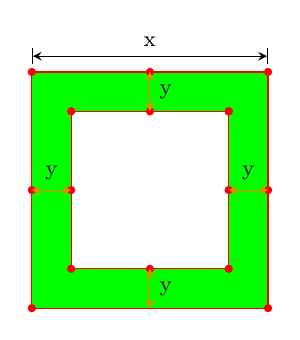
\begin{tikzpicture}[>=stealth,line join=round,line cap=round,font=\footnotesize,scale=1] \fill[green,draw=red] (0,0) rectangle (3,3); 
			\fill[white,draw=red] (0.5,0.5) rectangle (2.5,2.5); 
			\foreach \x/\y in {0/0,0.5/0.5,0/3,3/0,3/3,0.5/2.5,2.5,2.5,2.5/0.5,0/1.5,0.5/1.5,1.5/0.5,1.5/3,2.5/1.5,3/1.5,1.5/2.5}{\fill[red] (\x,\y) circle (1.5pt);} 
			\foreach \x/\y in {0/1.5,2.5/1.5}[\draw[<->,orange] (\x,\y)--++(0:0.5)node[midway,sloped,above,black]{y};] 
			\foreach \x/\y in {1.5/0,1.5/2.5}[\draw[<->,orange] (\x,\y)--++(90:0.5)node[midway,right,black]{y};] \draw[|<->|] (0,3.2)--(3,3.2)node[midway,sloped,above]{x}; 
		\end{tikzpicture}
	\end{center}
	\begin{enumerate}
		\item Viết biểu thức tính diện tích $S$ của đường bao quanh mảnh vườn theo $x$ và $y$.
		\item Phân tích $S$ thành nhân tử rồi tính $S$ khi $x=102$ m, $y=2$ m.
	\end{enumerate}
	
	\loigiai{
		\begin{enumerate}
			\item Diện tích của mảnh vườn hình vuông có độ dài cạnh bằng $x$ là $x^2$ (m$^2$).\\
			Diện tích phần còn lại của khu vườn hình vuông có độ dài cạnh bằng $y$ là $y^2$ (m$^2$).\\
			Diện tích $S$ của đường bao quanh mảnh vườn theo $x$ và $y$ là $S=x^2-y^2$  (m$^2$).
			\item $S=x^2-y^2=\left(x-y\right) \cdot \left(x+y\right)$.\\
			Thay $x=102$, $y=2$ vào biểu thức ta được: $S=\left(102-2\right) \cdot \left(102+2\right)=100 \cdot 104=10400$ (m$^2$).\\
		\end{enumerate}
	}
\end{vd}

\begin{vd}%[Dự án EX-9-Đề Cương Toán 8-L1]%[Phạm Hoàng Điệp]%[8D1H4-7]
	Cho $y>0$. Tìm độ dài cạnh của hình vuông có diện tích bằng $49y^2+28y+4$.
	\loigiai{
		Ta có $49y^2+28y+4=(7y)^2+2\cdot 7y\cdot 2+2^2=(7y+2)^2$.\\
		Vì $y>0$ nên $7y>0$, suy ra $7y+2>0$.\\
		Mà $49y^2+28y+4=(7y+2)^2$ là diện tích của hình vuông nên độ dài cạnh hình vuông bằng $7x+2$.
	}
\end{vd}

\subsubsection{Bài tập}

\begin{bt}%[Dự án EX-9-Đề Cương Toán 8-L1]%[Phạm Hoàng Điệp]%[8D1H4-7]
	Tìm một hình hộp chữ nhật có thể tích $2x^3-18x$ (với $x>3$) mà độ dài các cạnh đều là biểu thức chứa $x$.
	\loigiai{
		Ta có $2x^3-18x=2x\cdot \left(x^2-9\right)=2x(x+3)(x-3)$.\\
		Vì độ dài các cạnh của hình hộp chữ nhật đều là biểu thức chứa $x$ nên hình hộp chữ nhật có 3 kích thước cần tìm là $2x$, $x+3$ và $x-3$.
	}
\end{bt}

\begin{bt}%[Dự án EX-9-Đề Cương Toán 8-L1]%[Phạm Hoàng Điệp]%[8D1H4-7]
	\immini{Từ một miếng bìa có dạng hình tròn với bán kính $R$ (cm), bạn Hạnh khoét một hình tròn ở giữa có bán kính $r$ (cm) $(0<r<R)$ như hình bên.
		\begin{enumerate}
			\item Viết công thức tính diện tích phần còn lại của miếng bìa dưới dạng tích.
			\item Tính diện tích phần còn lại của miếng bìa, biết tổng hai bán kính là $10$ cm và hiệu hai bán kính là $3{,}5$ cm.
	\end{enumerate}}
	{\begin{tikzpicture}[line join=round,line cap=round,>=stealth,font=\footnotesize,scale=1]
			\def\r{2}
			\coordinate (O) at (0,0);
			\coordinate (A) at (-35:\r);
			\coordinate (B) at (180:\r-1);
			\draw[fill=orange!20] (\r,0) arc (0:360:\r);
			\draw[line width=1pt] (0,0) circle (\r);
			\draw[fill=white] (\r-1,0) arc (0:360:\r-1);
			\draw[line width=1pt] (0,0) circle (\r-1);
			\draw[<->,line width=0.8pt] (O)--(A);
			\draw[<->,line width=0.8pt] (O)--(B);
			\fill (O) circle (1.5pt);
			\coordinate [label=above:$r$,yshift=0pt,xshift=0pt] (C) at ($(B)!0.5!(O)$);
			\coordinate [label=above:$R$,yshift=0pt,xshift=0pt] (D) at ($(A)!0.6!(O)$);
	\end{tikzpicture}}
	\loigiai{
		\begin{enumerate}
			\item Diện tích miếng bìa hình tròn có bán kính $R$ là $\pi R^2$ (cm$^2$).\\
			Diện tích miếng bìa hình tròn bị khoét đi có bán kính $r$ là $\pi r^2$ (cm$^2$).\\
			Diện tích phần còn lại của miếng bìa là \[\pi R^2-\pi r^2=\pi\left(R^2-r^2\right)=\pi(R-r)(R+r)\,\,(\text{cm}^2).\]
			\item Diện tích phần còn lại của miếng bìa là $\pi(R-r)(R+r)=\pi\cdot3{,}5 \cdot 10=35\pi$ (cm$^2$).
		\end{enumerate}
	}
\end{bt}

\begin{bt}%[Dự án EX-9-Đề Cương Toán 8-L1]%[Phạm Hoàng Điệp]%[8D1H4-7]
	Bác Hoa gửi tiết kiệm $a$ đồng kì hạn $12$ tháng ở một ngân hàng với lãi suất $x\%$/năm.
	\begin{enumerate}
		\item Viết công thức tính số tiền bác Hoa có được sau $12$ tháng dưới dạng tích, biết bác Hoa không rút tiền ra khỏi ngân hàng trong $12$ tháng đó.
		\item Sau kì hạn $12$ tháng, tiền lãi của kì hạn đó được cộng vào tiền vốn, rồi bác Hoa tiếp tục đem gửi cho kì hạn $12$ tháng tiếp theo. Viết công thức tính tổng số tiền mà bác Hoa nhận được sau khi gửi $24$ tháng trên dưới dạng tích, biết trong $24$ tháng đó, lãi suất ngân hàng không thay đổi và bác Hoa không rút tiền ra khỏi ngân hàng.
	\end{enumerate}
	\loigiai{
		\begin{enumerate}
			\item Số tiền bác Hoa có được sau $12$ tháng là $a+a\cdot x\%=a(1+x\%)$ đồng.
			\item Số tiền bác Hoa có được sau $24$ tháng là \[a(1+x\%)+a(1+x\%)\cdot x\%=a(1+x\%)(1+x\%)=a(1+x\%)^2 \ \text{ (đồng)}.\]
		\end{enumerate}
	}
\end{bt}

\begin{bt}%[Dự án EX-9-Đề Cương Toán 8-L1]%[Phạm Hoàng Điệp]%[8D1H4-7]
	Một mảnh vườn có dạng hình chữ nhật với chiều rộng là $x$ (m), chiều dài là $y$ (m).
	\begin{enumerate}
		\item Viết đa thức biểu thị diện tích của mảnh vườn.
		\item Nếu tăng chiều rộng lên $4$ m và giảm chiều dài đi $5$ m thì được mảnh vườn mới. Viết đa thức biểu thị diện tích của mảnh vườn mới.
		\item Viết đa thức biểu thị phần diện tích chênh lệch của mảnh vườn mới so với mảnh vườn ban đầu.
	\end{enumerate}
	\loigiai{
		\begin{enumerate}
			\item Diện tích hình chữ nhật là $S=x\cdot y$ (m$^2$).
			\item \begin{itemize}
				\item Tăng chiều rộng thêm $4$ m suy ra $x+4$ (m).
				\item Giảm chiều dài đi $5$ m suy ra $y-5$ (m).
			\end{itemize}
			Vậy diện tích mới là $S'=(x+4)(y-5)$ (m$^2$).
			\item Diện tích mới lớn hơn so với diện tích cũ là \begin{eqnarray*}
				S''=S'-S &=&(x+4)(y-5)-xy\\
				&=&xy-5x+4y-20-xy\\
				&=&-5x+4y-20 \, (\text{m}^2).
			\end{eqnarray*}
			Vậy biểu thức phần diện tích lớn hơn là $S''=-5x+4y-20$ (m$^2$).
		\end{enumerate}
	}
\end{bt}


